Scaling up a DDMS requires not only storing progressively more data, but also a dramatic increase in computing resources.  As alluded to in Section \ref{sec:storage}, DDMS and their corresponding transition programs are amenable to having their data distributed across a cluster: (1) The only data structures used by transition programs are maps, which are amenable to horizontal partitioning.  (2) At the granularity of a single update, iterative computations are completely data-parallel.  (3) The effect of a sequence of updates (i.e., executing the corresponding trigger functions) is independent of the order in which the updates are applied.

\parheading{Order of Execution}
Though order of execution is irrelevant at the granularity of updates, transition functions are constructed under the assumption that they are operating on a \textit{consistent} snapshot of the DDBS's state.  \todo{Example here?}  Thus, the entire sequence of instructions composing the trigger function must be executed atomically.  Ensuring this atomicity property is the first of the two core challenges we have encountered in constructing a distributed DDBS runtime.

\parheading{Distribution}
Each update in our distributed DDBS runtime design employs three classes of actors:
\begin{itemize}
\item \textit{source nodes}: Nodes hosting maps read by the update's trigger function (maps appearing on the right-hand side of the function's statements).
\item \textit{computation nodes}: The node or nodes where each computation is performed.
\item \textit{destination nodes}: Nodes hosting maps written to by the update's trigger function (maps appearing on the left-hand side of the function's statements).
\end{itemize}
Note that these actors are logical entities; It is not necessary (and in fact detrimental) for each actor to be placed on separate physical hardware.  However, making these distinctions allows us to better understand the tradeoffs involved in the second distributed DDBS core challenge: selecting an effective partitioning scheme.  

\subsection{Execution Models}
We first address the issue of atomicity.  We provide two mechanisms: one for providing a serial execution environment for transition programs, and a more efficient approach to providing the illusion thereof.

\parheading{Serial Execution}
The most straightforward way of achieving atomicity is to ensure serial trigger function execution.  Requiring all nodes in the cluster to block on a barrier after every update is unscalable.  However, a similar effect can be achieved more efficiently by using finer-grained barriers; Each update is processed by first notifying each of its destination nodes of an impending write.  Reads at the update's source nodes are blocked while writes from prior updates are pending.

Nodes across the cluster must agree on the relative ordering of updates.  An update ordering may be obtained from the update source (e.g., if the cluster is accepting inputs from a single source, such as in a data warehouse live-mirroring an OLTP database), from a central coordinator (e.g. as in \cite{peng-incremental:10}), or by some form of distributed consensus protocol (e.g., by using local timestamps at each update producer and a deterministic tiebreaker like an ip address).

Also necessary is a mechanism for ensuring consistent delivery of updates from separate input sources; Before completing a read, source nodes must not only ensure that all prior pending writes have been completed, but also that all notifications for prior updates have been received.  A simple solution is to channel all updates through a single server -- this has the advantage of also providing a global ordering over all updates.  However this solution creates a scalability bottleneck.  Alternative solutions like broadcasting updates or periodic commits are possible, but introduce considerable synchronization overheads.

\parheading{Speculative Execution}
As an alternative, we can optimistically perform reads immediately, without blocking -- at least without blocking on the possibility that a write could potentially occur.  Though doing so avoids significant synchronization overheads, it introduces the possibility of inter-update conflicts and the corresponding need for corrective mechanisms.  

Fortunately, the points of conflict in a transition program are easily identified.  Furthermore, because write operations are limited to additive deltas, there is a clear mechanism for composing writes, even when applied out of order.

We supplement maps with two additional data structures, as illustrated in Figure \ref{fig:speculativeStorage}.  (1) Source nodes maintain a record of all read operations.  (2) Destination nodes record each write operation independently; map entries are stored as histories rather than single values.  Each operation is tagged with and sorted by a timestamp \texttt{<t>} representing the operation's position in the global order of updates.

\begin{figure}
\begin{center}
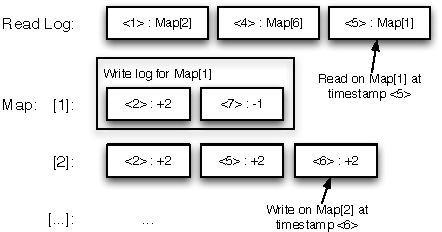
\includegraphics[width=3.0in]{graphics/speculative_storage}
\end{center}
\caption{Supplemental data structures used to facilitate speculative execution in a distributed DDBS.}
\label{fig:speculativeStorage}
\end{figure}

In the case of an out-of-order read operation (i.e., one that arrives after a write operation that logically precedes it), the write history us to reconstruct the state of the map at an earlier point in time.  In the case of an out-of-order write operation, the read record allows us to send a \textit{corrective update} to each computation node affected by the write.

Both data structures grow over time.  To prevent unbounded memory usage, it is necessary to periodically truncate, or garbage collect the entries in each.  This in turn, requires the runtime to periodically identify a cutoff point; the ``last" update for which there are no operations pending within the cluster.  The read history is truncated at this point, and all writes before this point are coalesced into a single entry.  Though this process is slow, it does not interfere with any node's normal operations, and can be performed infrequently; Once every few seconds is reasonable.

A potential drawback of the speculative execution model is that it produces eventual consistent results; Unless the system quiesces, there is no guarantee that the sum of all entries in the write history of the result map will be representative of the actual query results at some point in the update stream.  However, a side effect of the garbage collection process is that each garbage collection run, in effect generates a consistent snapshot of the system.  As in other eventual consistency systems\cite{bayou}, this approach offers a Hybrid consistency model: The same infrastructure produces both low-latency eventually consistent results, as well as higher-latency consistent snapshots.

\subsection{Partitioning Schemes}
The second challenge associated with distributing a transition program across the cluster is the distribution of logical nodes (source, computation, and destination) across physical hardware in the cluster.  In addition to more complex, min-cut based partitioning schemes for the data, DBToaster considers two simple partitioning heuristics for distributing computation: (1) compute the data where it will be stored, or (2) store the data where it will be used.  

\parheading{Destination-Computation}
Given the one-to-one correspondence between computation nodes and destination nodes, the simplest partitioning scheme is to perform computations where the data will be stored -- that is, the destination and computation nodes are co-located.  As part of update evaluation, each source node transmits all relevant map entries to the destination node.  Upon arrival, the destination node evaluates the statement and stores the relevant results.

\parheading{Source-Computation}
Though simple, transmitting every relevant map entry with every update can be wasteful, especially if the input map entries don't change frequently.  An alternative approach is to co-locate all of the source nodes and the computation node.  When evaluating an update, the computation can be performed instantaneously, and the only overhead is transmitting the result(s) to the destination node(s).  This is particularly effective in queries where update effects are small (e.g., queries consisting mostly of equijoins on key columns).

However, this approach introduces an additional complication.  It is typically not possible to generate a partitioning of the data that ensures that for each statement in a trigger program, all the source nodes will be co-located.  In order to achieve a partitioning, data must be replicated; each map is stored on multiple physical nodes.  While replication is typically a desirable characteristic, storage-constrained infrastructures may need to use a more complex partitioning scheme.

